\subsection{Mayo Clinic CT Dataset}

\begin{frame}{Mayo Clinic CT Dataset}
  \begin{itemize}
    \item Released by the \textbf{Mayo Clinic} for research purposes.
    \item Contains chest \textbf{Computed Tomography (CT)} scans.
    \item Images are in \textbf{grayscale (black and white)} format.
    \item Focus on \textbf{lung nodules} and early detection of \textbf{lung cancer}.
    \item Widely used in machine learning and AI medical imaging research.
  \end{itemize}
  \vspace{0.5cm}
  \begin{center}
    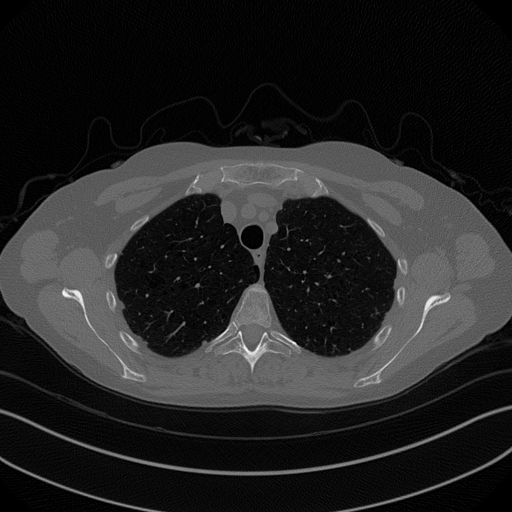
\includegraphics[width=0.25\linewidth]{media/2.png}
    \hspace{0.3cm}
    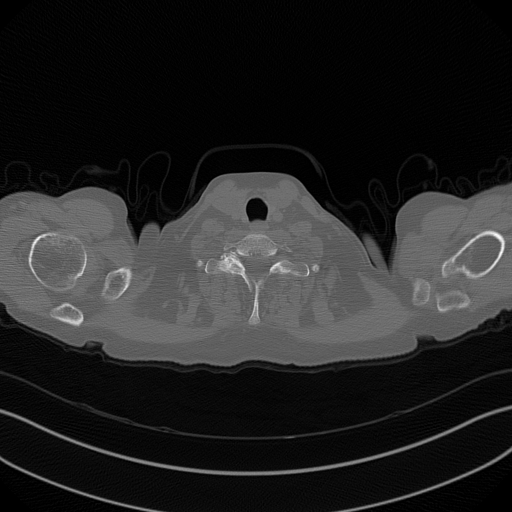
\includegraphics[width=0.25\linewidth]{media/3.png}
    \hspace{0.3cm}
    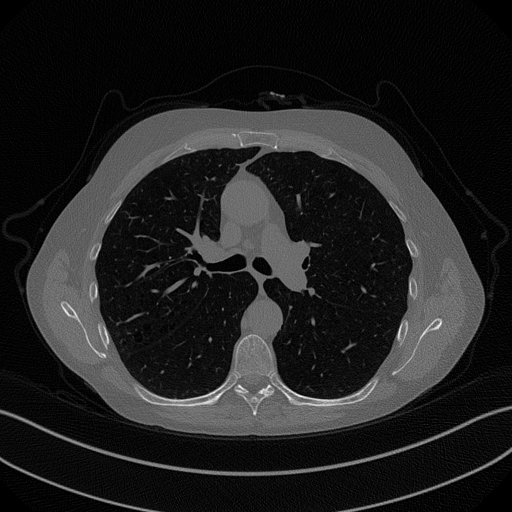
\includegraphics[width=0.25\linewidth]{media/100.png}
  \end{center}
\end{frame}

\begin{frame}{Preprocessing and Augmentation}
  \begin{itemize}
    \item All CT images were preprocessed and resized to a fixed dimension of \textbf{128 × 128 pixels}.
    \item This standardization ensures consistency for input into deep learning models.
    \item The dataset was \textbf{augmented} to avoid overfitting and improve model generalization (detailed later).
  \end{itemize}
\end{frame}